\lettrine{T}{he question this study attempts to answer}, is whether linkages to China can have an impact on freedom of expression in other countries or not.  Before being able to answer the main research question, we need to look at the context around freedom of expression. We need to given an answer to two important preconditions: why freedom of expression is important,  and in what context it is relevant. Freedom of expression is, of course, important in and of itself, but it also important for democracy more specifically.  

I start this chapter with a closer look at what freedom of expression entails, how we might be able to define it, and why it is important.  I draw on the theories of thinkers such as John Stuart Mill to argue the importance of freedom of expression and its limitations.

After defining freedom of expression, I go on to place it in the context of democratisation and autocratisation, and explicate on why exactly the freedom of expression is important when defining autocracy. Specifically, I focus on the definition given by Robert A. Dahl and how, for him, freedom of expression is an essential feature of his definition of democracy. The next couple of sections narrows down the overarching theme of autocratisation, by looking at factors that might help explain autocratisation. Many of these are well studied, but one factor---autocratic diffusion---is, as of yet, not well enough understood. 

Within the framework of diffusion theory, I further narrow the theme down to a theory about leverage and linkages developed by \citet{levitsky_linkage_2006}. I hypothesis that this might be an important explanation, among others, for the great variation we see in the level of freedom of expression people enjoy around the world. The nuts-and-bolts of this hypothesis is described more thoroughly in the theory chapter, but this section should serve to help the reader understand the ground I am working on. 

\section{Freedom of expression}
Freedom of expression is the dependent variable in this study, and we should therefore examine it in some detail. This section will look at freedom of expression in isolation, while the subsequent sections will place it in a context of democracy and its waning in recent years. 

Freedom of expression is one of the most fundamental freedoms of human beings. \citet{amnesty_international_freedom_2023} on their webpage writes that `Freedom of expression also underpins other human rights [...] and allows them to flourish.'  It is a defence and guarantor of other freedoms: like freedom of conscience, freedom of religion, freedom of the press, freedom of assembly, among many others. It is exactly this fundamentality that makes freedom of expression important to study.

Even from early on, freedom of expression has been associated with two major positive attributes: the search for truth and self-improvement \citep[pp. 25-80]{mill_liberty_2010}. Without freedom of expression, ideas cannot clash to discover what is the whole of `truth' and people cannot develop the necessary understanding of these truths. Mill argued the importance of the right to express one's opinions all the way back in 1859, and while freedom of expression in most parts of the world have steadily increased, it is still not a secure right. Even in Western societies where freedom of expression has been a keystone of the liberal way of life, it has at points in time, even at present, been threatened. Mill was an optimist at this point, writing that: `The time, it is to be hoped, is gone by, when any defence would be necessary of the "liberty of the press" as one of the securities against corrupt or tyrannical government.'  \citep[p. 25]{mill_liberty_2010} He was, unfortunately, mistaken at this point. 

The impact freedom of expression has on society is also what makes it so relevant to the topic of autocratisation. If a regime denies its citizens the freedom to express themselves; to communicate their ideas and preferences openly and without fear, democracy cannot flourish. For democracy to function, people need to be informed about the `true' state of affairs. And since there is no objective truth shared by all people, each and everyone must be allowed to express their opinions on all matters. By so doing, a society may build a consensus of what is the true state of the world, at least to some degree. 

While freedom of expression is a fundamental right, there are in most societies limits to this freedom \citep{bonotti_freedom_2021}. The freedom to express oneself is a powerful tool, and rightly feared by regimes of both democratic and authoritarian dispositions. Sometimes the reasons are the same; sometimes they diverge. Threats to specific people or groups are generally not allowed in either regime types. The same with libel, and other acts of targeted use of `expression' for violence or hurt. For authoritarian regimes, the freedom of expression constitute a very fundamental threat to their rule. If people are allowed to express themselves freely, they might demand a different, usually a democratic regime. A democratic regime on the other hand, would fear that pernicious actors should take control of the \textit{vox populi} and use it to remove the freedoms that are so vital to the citizens, and even to the actor's own success. This was of course what happened in Weimar-Germany, and this specific lesson, it seems, must unfortunately be relearned even today. 

There is also evidence that the freedom of expression is under pressure. The Varieties of Democracy Institute (henceforth the V-Dem institute) release an annual report on the state of democracy in the world. In this release they show a figure of the 20 indicators that have declined the most over a ten year period, reproduced here in Figure \ref{fig:declining}. Of these 20 indicators eight are indicators of freedom of expression, five of the top ten are, and lastly the top three are all related to freedom of expression. There should thus not be any question that freedom of expression has declined in recent years.

\begin{figure}[hbt!]
    \centering
    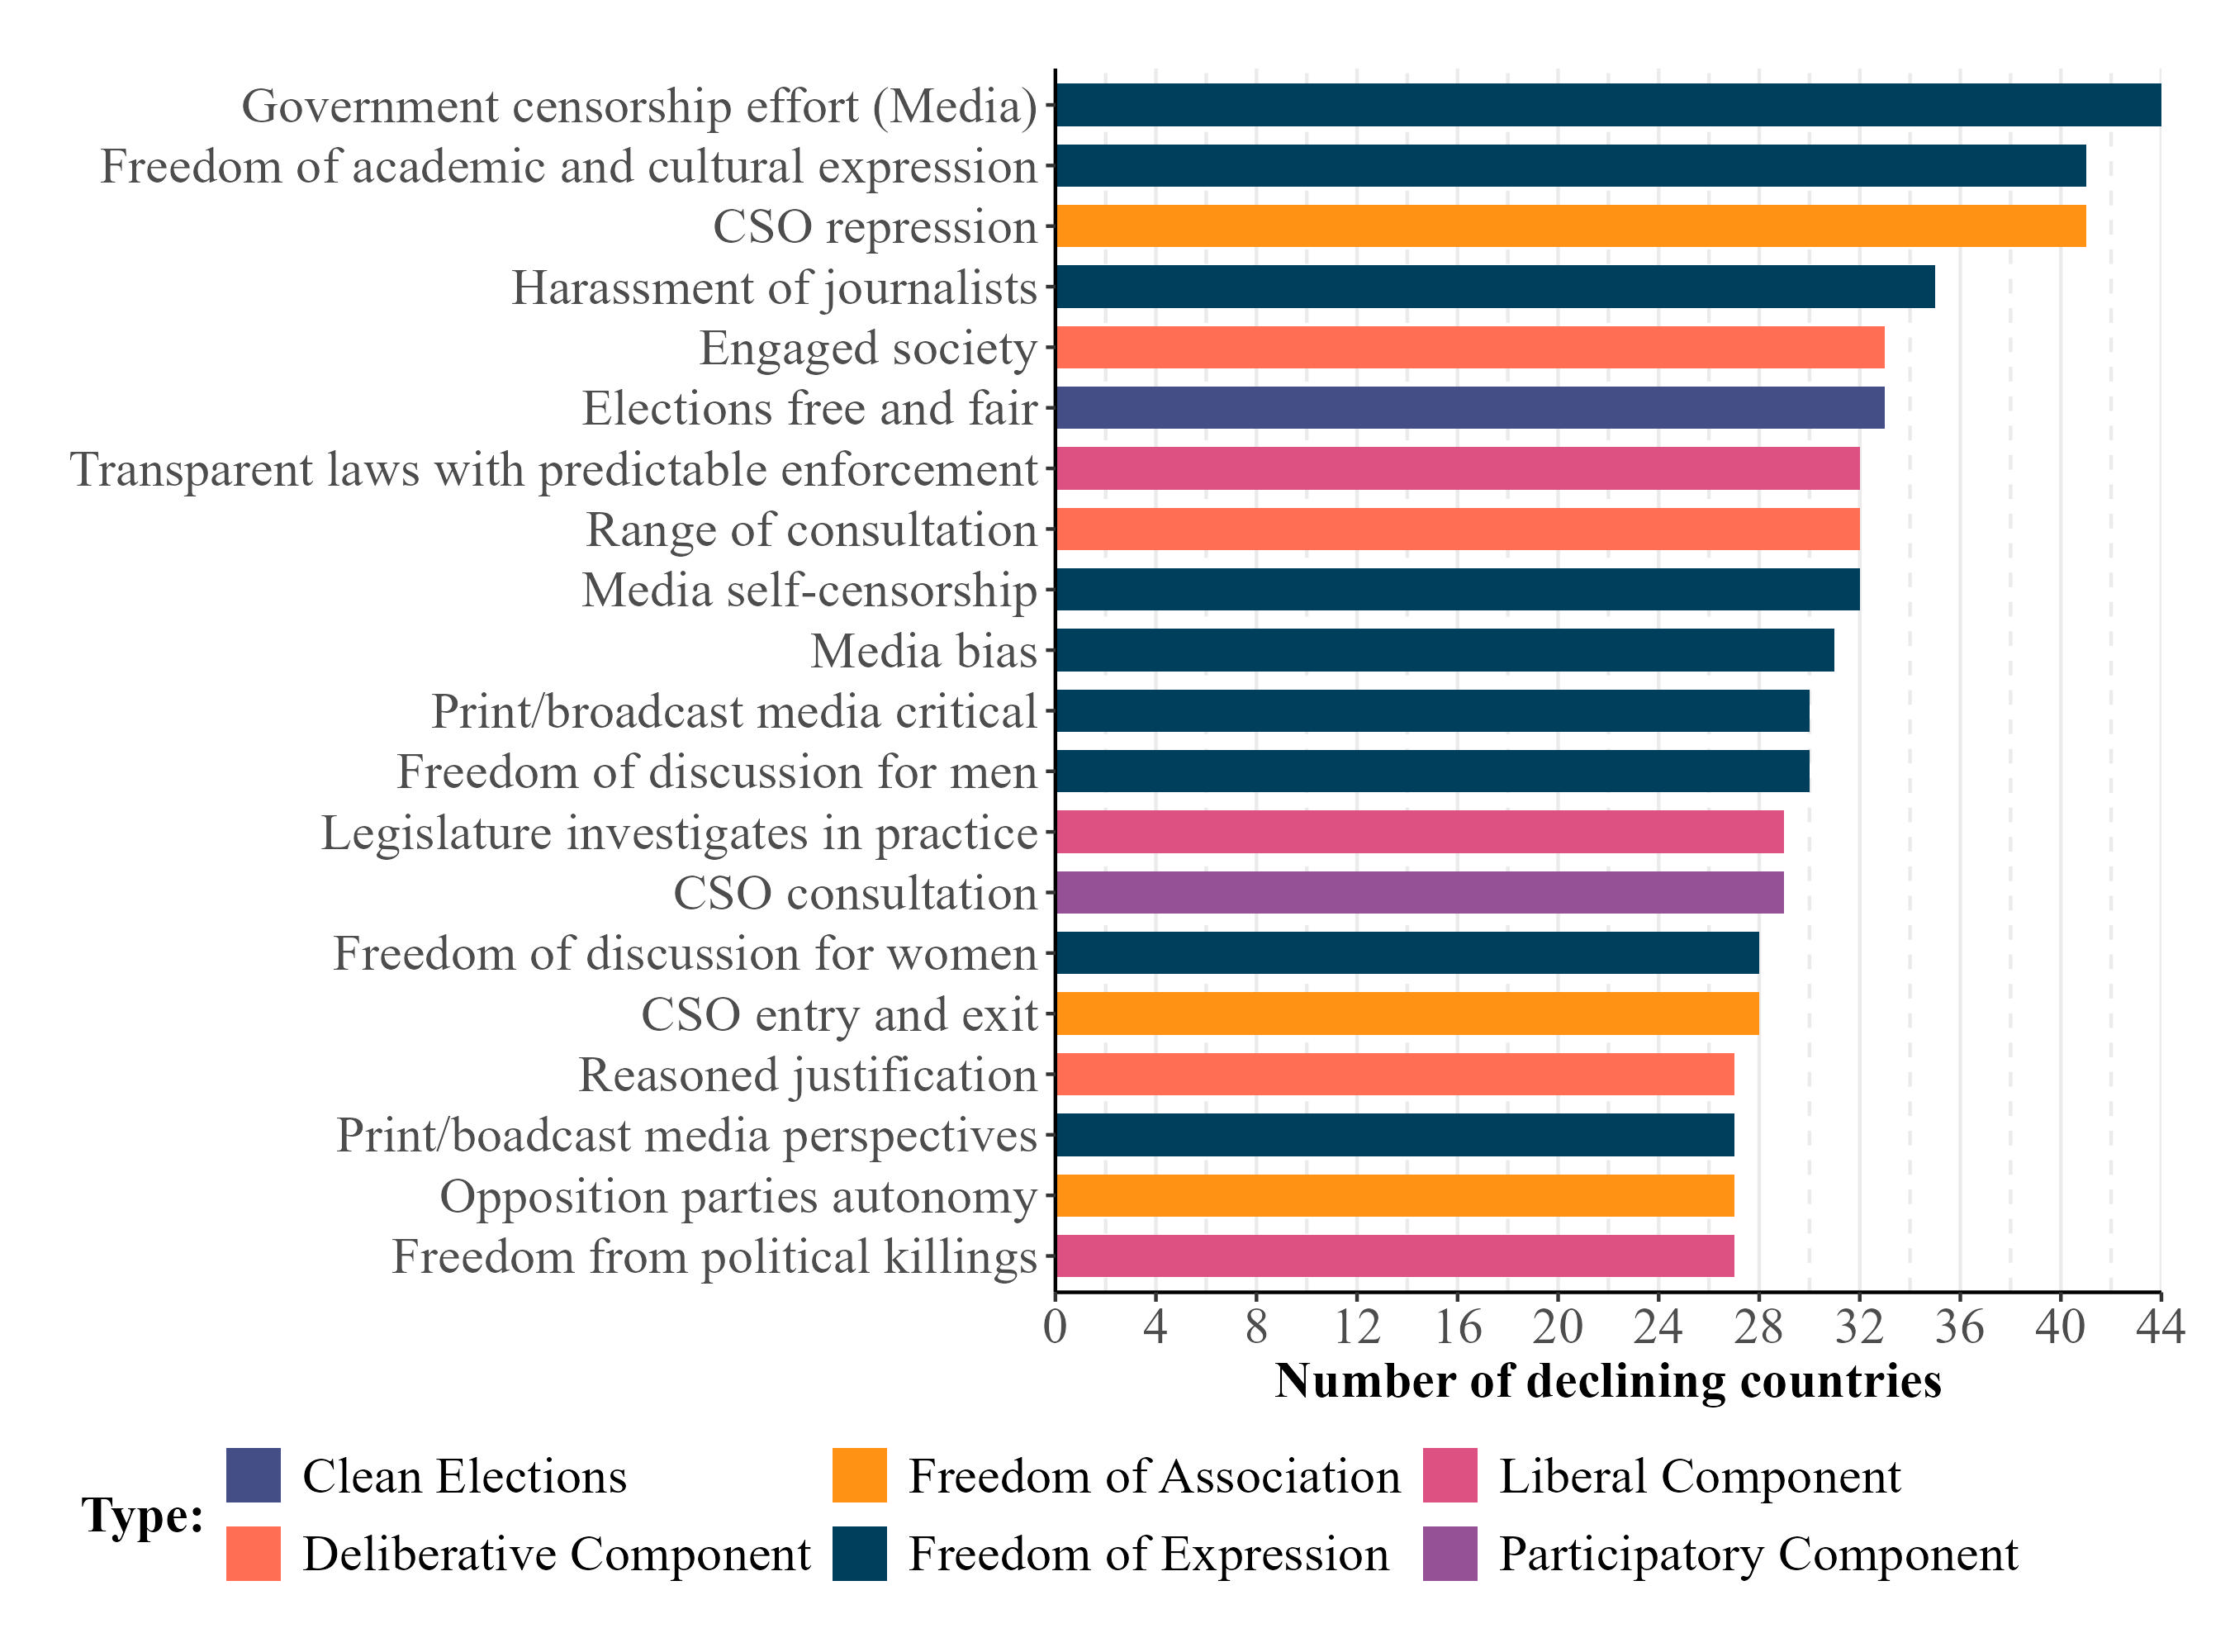
\includegraphics[width=\linewidth]{graphics/declining_indicators.jpeg}
    \caption{Top-20 declining indicators 2013-2023 \citep[p. 17]{nord_democracy_2025}}
    \label{fig:declining}
\end{figure}

Since freedom of expression, as I have accounted for above, is integral to any rigorous definition of autocracy, it is important to look at this variable in isolation, as connections between other variables and the level of democracy might be obscured by improvements in other indicators.

\section{Defining Autocracy}
Autocracy is most often identified in the negative---the absence of fundamental components of democracy---and our discussion of autocracy should thus start by defining democracy. Of course, this is far from easy, as democracy in the modern world is often given a complex definition so as to encompass whatever concept is normatively fashionable, often stretching the concept such as to be conflated with other near-lying concepts, most notably liberalism.

A popular way to avoid the problem of conceptual stretching is to use a minimal definition of democracy.\footnote{The problem of conceptual stretching is a considerable one when defining democracy, however, as there is no room for a lengthier discussion of this, I will restrict myself to point out some well articulated viewpoints on the matter: \citealp[see:][]{sartori_concept_1970, collier_conceptual_1993} for a discussion of concepts, and for democracy in particular, \citealp[see:][]{collier_democracy_1997}.} This can of course be done by using the plane meaning of the word: rule by the people. This might seem a good enough definition for some, however, the statement is far too broad to be useful in a scientific context. Questions such as how is this power executed and how the decisions are made naturally comes to mind. The next section makes clear what is meant by democracy and autocracy going forward.

Two famous definitions have been put forward by scholars of political science. The first one articulated was that by Joseph A. Schumpeter in his classic 1943 book \textit{Capitalism, Socialism and Democracy} \citeyearpar{schumpeter_capitalism_2010}.  Schumpeter argues that `the democratic method is that institutional arrangement for arriving at political decisions in which individuals acquire the power to decide by means of a competitive struggle for the people’s vote' \citep[p. 241]{schumpeter_capitalism_2010}. Schumpeter sees the connection between democracy and freedom of expression as important, but not a defining part of what democracy is \citep[pp. 243-244]{schumpeter_capitalism_2010}. Schumpeter's view has been adopted and explicated on by several other scholars, notable among them is Przeworski who established a list of three features necessary for a to achieve `contestation'---the minimal point to which democracy is reducible. The three features are as follows: uncertainty of the outcome, that the outcome is irreversible, and that elections are repeated (\citeauthor{przeworski_democracy_1991} \citeyear{przeworski_democracy_1991}, pp. 10-14; \citeauthor{przeworski_modernization_1997} \citeyear{przeworski_modernization_1997}, pp. 14-18). The advantage of this approach is that it forms a concept that is highly differentiated and allows for a dichotomous definition of democracy and autocracy. 

A second, famous definition of democracy is that by Robert A. Dahl, first fleshed out in his 1971 book \textit{Polyarchy} \citeyearpar{dahl_polyarchy_1971}. Dahl's notion of polyarchy \footnote{Dahl uses the word polyarchy in stead of democracy, as he defines democracy to be an ideal type \citep[p.9]{dahl_polyarchy_1971}.} has two principal components, contestation and suffrage. Suffrage is what part of the population has the right to vote. In the early democracies this was a considerable restriction, however, in today's democracies, this right is usually given to every citizen above a certain age-threshold. Although important, it is less consequential to this study, as suffrage is very nearly universal. The second component is much more interesting for the study of contemporary democracies. Contestation is whether or not the elections are `real'. What I mean by this is: are the elections fair and consequential; is change possible? 

This type of system, polyarchy, can only come about if citizens have the opportunity to (1) formulate their preferences, (2) signify their preferences, and (3) have preferences weighted equally in conduct of government \citep[pp.2-3]{dahl_polyarchy_1971}. To achieve this, Dahl also includes a list of seven institutions and five criteria for a democracy that can be seen in Figure \ref{tab:dahl} 

\begin{table}[hbt!]
\centering
\caption{\label{tab:dahl}Dahl's list of institutions and criteria}
\begin{tabularx}{\textwidth} {
    >{\raggedright\arraybackslash}X
    >{\raggedright\arraybackslash}X}
\toprule
The following institutions... & are necessary to satisfy the following criteria \\
\midrule
1. Elected officials & \\
2. Free and fair elections & I. Voting equality \\
& \\
1. Elected officials & \\
3. Inclusive Suffrage & \\
4. Right to run for office & \\
\cellcolor[HTML]{003F5C}\textcolor{white}{5. Freedom of expression} & \\
6. Alternative information & \\
7. Associational autonomy & II. Effective participation \\
& \\
\cellcolor[HTML]{003F5C}\textcolor{white}{5. Freedom of expression}  \\
6. Alternative information & \\
7. Associational autonomy & III. Enlightened understanding \\
& \\
1. Elected officials & \\
2. Free and fair elections & \\
3. Inclusive Suffrage & \\
4. Right to run for office & \\
\cellcolor[HTML]{003F5C}\textcolor{white}{5. Freedom of expression}  & \\
6. Alternative information & \\
7. Associational autonomy & IV. Control of the agenda \\
& \\
3. Inclusive Suffrage & \\
4. Right to run for office & \\
\cellcolor[HTML]{003F5C}\textcolor{white}{5. Freedom of expression}  & \\
6. Alternative information & \\
7. Associational autonomy & V. Inclusion \\
\bottomrule
\multicolumn{2}{l}{\raggedright{\textit{Table copied from \citet{dahl_democracy_1989}, emphases are my own.}}}
\end{tabularx}
\end{table}



The requirements touch on different aspects of the process, like institutions for competition and making preferences actual policy, but for our more narrow discussion, quite a number of these requirements concerns the construction and articulation of preferences; for which freedom of expression is absolutely necessary.

Dahl's definition of democracy seem to me to be closer to my own conception of the word. Democracy in a perfect world would probably only need to be defined in minimalistic terms, however, without the possibility to fairly contest an election and create and make known one's preferences, democracy would be a hollow thing indeed. When citizens do not have the freedom to hear or form opposing views of whatever regime is in place, contestation is imperfect. Dahl's definition also has another advantage, which is that it better captures the different degrees of how authoritarian a regime is. It might be a less differentiated concept than a minimal definition, however, since the world---and even more so the social world---is rarely possible to divide into neat and absolute categories, this better captures the complexity of real life. China and Singapore might serve as examples of this. Both regimes are authoritarian, but the average citizen have much more input on the governance of the country in Singapore than in China. 

Having defined democracy, there is not too much more we need to be able to define autocracy. Autocracies are a diverse selection of regime types united only by the fact that they have major failures when it comes to the five criteria and seven institutions of Dahl. Failure to live up to the `ideal' on all is not necessary, all countries have some restrictions on everything from the officials to the freedom of association, but major discrepancies on one or more might allow us to classify it as an autocracy. This definition of autocracy also makes it quite hard to dichotomise, and a country can be more or less autocratic, according to what criteria the regime fulfil or not.\footnote{One might distinguish between run-of-the-mill authoritarian regimes or totalitarian ones. Not dissimilar to democracies, authoritarian regimes might get their own adjectives to distinguish larger or smaller differences \citep{collier_democracy_1997}, however, this is not a discussion which will be continued here.}

We have in this section taken a closer look at the definition of democracy and autocracy and have come to the conclusion that an autocracy is the absence of certain criteria, notable among them is freedom of expression. This is the definition that will be used henceforth as we pivot to look at autocratisation. 

\section{Autocratisation}
Samuel P. Huntington's \textit{The third way} \citeyearpar{huntington_third_1991} was a game changer in the study of democratisation. Huntington conceptualised democracy occurring in waves---periods in time where several countries turned democratic all at once. When he was writing in the late 1980's and the first years of the 1990's, he could not have known that the third wave would continue for several more years after that point. However, Huntington rightly saw in the data a second `type' of wave, a reversed wave of democratisation, and he also saw the beginning of the third  reverse wave, or as we better know it today, the third wave of autocratisation.

\begin{figure}[hbt!]
\centering
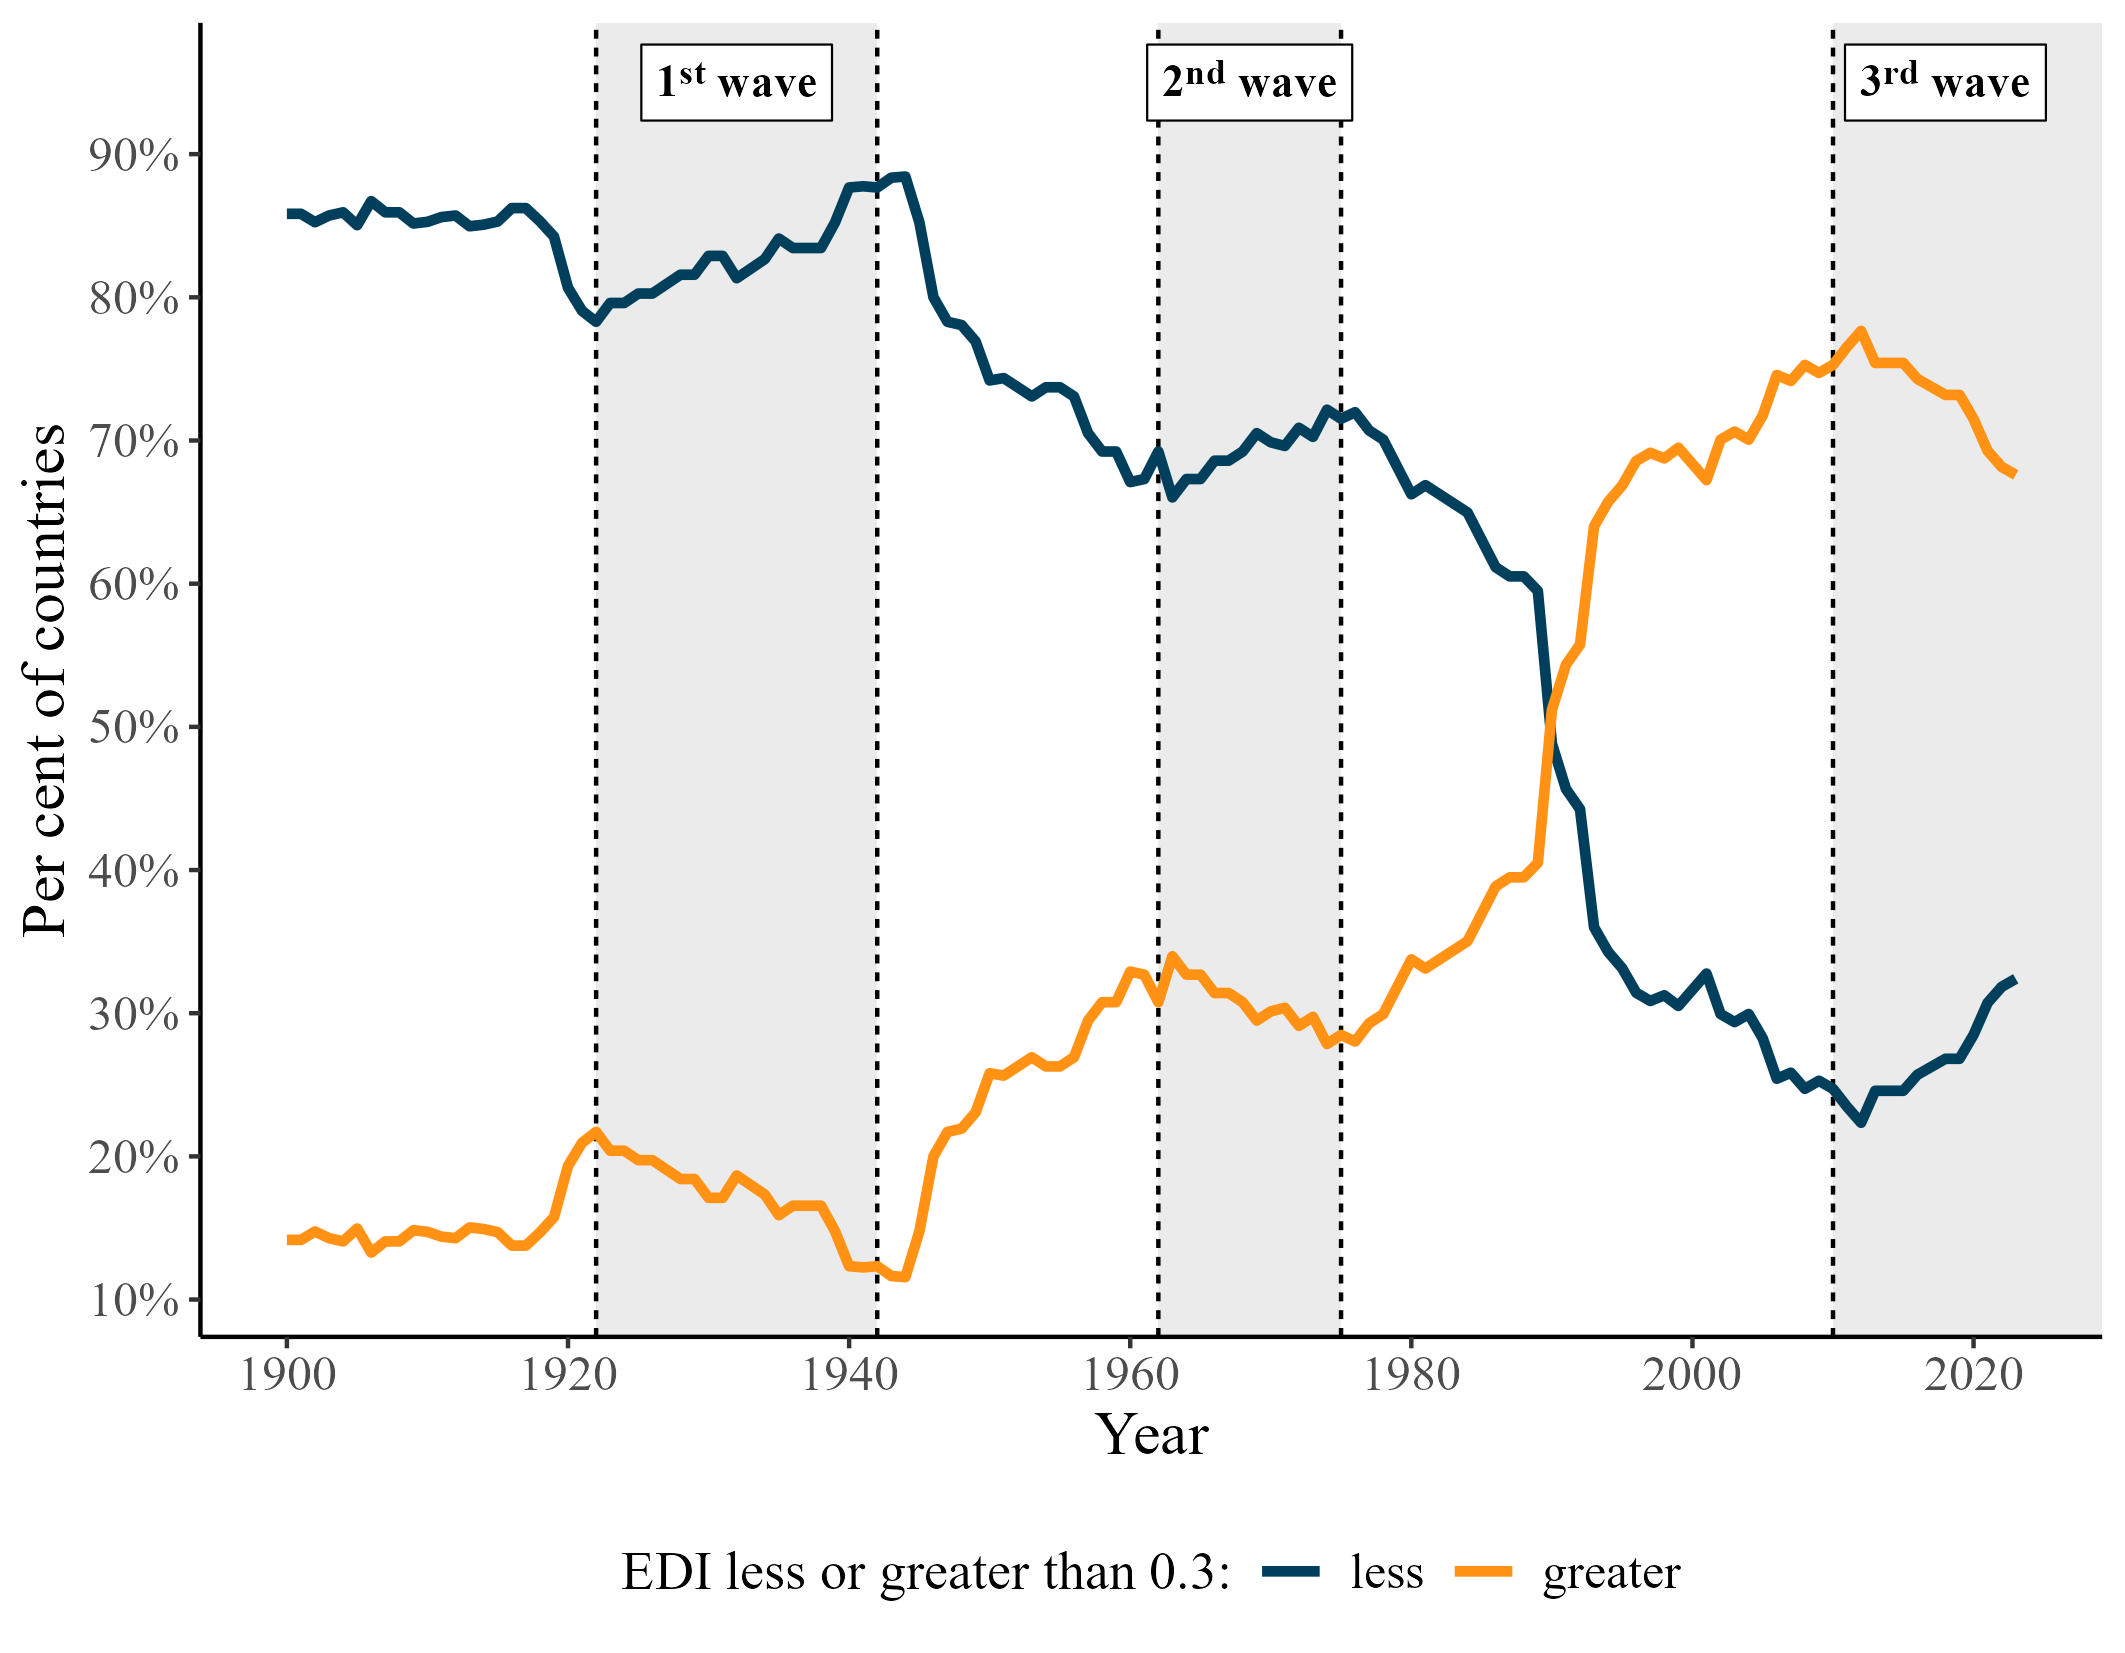
\includegraphics[width = \textwidth]{waves.jpeg}
\caption{\label{fig:autocratisation}The three waves of autocratisation}
\end{figure}

Using the V-Dem institute's Electoral Democracy Index (EDI) \footnote{This is a part of the varieties of democracy dataset \citep{coppedge_v-dem_2025}.}, Figure \ref{fig:autocratisation} shows the proportion of countries with an EDI score greater or less than 0.3. The index is measured from zero to one; however, as the scores are very low for most countries, a threshold of 0.5 would historically be far too high to see evidence of Huntington's waves. The grey fields on Figure \ref{fig:autocratisation} show when the waves of autocratisation are taking place. The dates of the first two waves are roughly taken from \citet[p.16]{huntington_third_1991} , the date of the third wave is placed similar to the two first waves, at the point where the number of countries with an EDI score below 0.3 begins to grow. Today we are still near an all-time high, however, the decline has been noticeable. 

As can be seen from Figure \ref{fig:autocratisation} authoritarian regimes are on the rise after a long period of decline. A similar figure appears in \citet{luhrmann_third_2019}, but with slightly differing dating of the waves. Scholars are now furiously debating how and why the current wave of autocratisation is happening.  The process is being described as a slow one, legitimised by the very institutions of democracy \citep{varol_stealth_2015, bermeo_democratic_2016, luhrmann_third_2019}. This is markedly different from previous waves of autocratisation that were more dramatic \citep[pp. 6-8]{bermeo_democratic_2016}, often involving the military. What has also worried proponents of democracy is the fact that a larger part of the autocratising countries have been consolidated democracies \citep{luhrmann_third_2019}. 

Much research has also been done on the processes by which they happen. The reasons can be divided into two categories by the main factor: domestic or external; where the former is far more widely discussed than the latter. The domestic factor will be discussed in this section, and it is also going to touch on some ancillary external factors. The focus of this thesis is not domestic factors, however, we cannot disregard that these variables have an influence on the state of democracy in a country, some of which may possibly have an effect on the the extent to which a population enjoys the rights accorded to them in free societies. The main discussion of external factors will come in the section below.

\subsection{Domestic Factors of Autocratisation}
Economic prosperity and democracy goes hand in hand. This is most famously explicated on by \citet{lipset_social_1959} in what has now become known as \textit{modernisation theory}, which sees economic development as a necessary precursor for the development of democracy. As the third wave of democratisation has created a lot of new democracies, it would not be unreasonable to think that some of the poorer countries will revert, as they do not have the resources to maintain a democratic system of government. Lipset's theory has had its fair share of critics, but even in spite of aberrations like Turkey's backsliding in the late 2010's, new studies shows evidence that the correlation between economic development and democracy is still very robust \citep{brownlee_limited_2017}.

Similar to modernisation theory, there is evidence that economic grievances, like generation differences caused by financial depressions \citep[pp. 132-174]{norris_cultural_2019}, losing out on globalisation \citep{ballard-rosa_economic_2021}, and missing out on the growth in home prices \citep{ansell_sheltering_2022}, has had an effect on the peoples commitment to democratic values. This is not universally accepted as some argue that economic factors only constitute a small part of the equation \citep{margalit_economic_2019}.

According to \citet{margalit_economic_2019} cultural factors plays an even bigger part in explaining peoples commitment to democratic values, and this has received much support. All the way back to !Weber! cultural factors have been suggested to influence the likelihood of a country becoming democratic. Religion \citep[pp.72-85]{huntington_third_1991}, immigration (\citeauthor{dinas_waking_2019} \citeyear{dinas_waking_2019}; \citeauthor{norris_cultural_2019} \citeyear{norris_cultural_2019}, pp.~175-212), intergenerational differences \citep{foa_youth_2020, foa_danger_2016, norris_cultural_2019, wuttke_have_2022}, majoritarianism \citep{grossman_majoritarian_2022, wunsch_demand_2023}, and party identity \citep{abramowitz_united_2019, bisgaard_how_2019, graham_democracy_2020, iyengar_strengthening_2018, krishnarajan_rationalizing_2023, peterson_partisan_2021, singer_fiddling_2023} have all been suggested to influence peoples commitment to democratic values, however, no consensus has emerged and some of the findings are contradictory (see for instance \citeauthor{schafer_cultural_2022} \citeyear{schafer_cultural_2022} for a rebuttal of \citeauthor{norris_cultural_2019} \citeyear{norris_cultural_2019}). 

The finger has also been pointed at elites and their actions. Political parties have been critiqued for lacking responsiveness to the demands of their constituents or opening the field to populist \citep{berman_causes_2021, grzymala-busse_failure_2019}. Others have indicated that elite behaviour can influence the electorate \citep{broockman_causal_2017, clayton_elite_2021}, and thereby undermine democratic norms.

Domestic factors are important for explaining autocratisation, but there is no agreement as to what extent domestic factors alone can be said to drive the current wave of autocratisation. A different approach might help us explain the phenomenon more thoroughly, which to look at exogenous factors.

\subsection{International Factors of Autocratisation}
The international element has always been a part of the field of studies on democracy. The first trial run of democracy in ancient Athens was ended in part by international factors. According to Thucydides, the oligarchic coup that brought down Athenian democracy in 411 BCE was ostensibly caused by Persian support of Alcibiades, a would-be demagogue \citep[pp. 562-599]{thucydides_history_1972}.\footnote{Alcibiades himself was not part of the actual coup, however, he had convinced powerful Athenians that Persian aid would not be forthcoming unless they abolished democracy, as the Persians considered democracies to be untrustworthy and only Alcibiades could regain Persian trust. In the end the Persians were more interested in playing Athens and Sparta against each other, and Alcibiades, in a twist of fate, became a saviour of Athenian democracy.}

The most obvious way for a foreign country to affect democracy in a country is by simply conquering it. If you were to look at a map showing the level of democracy in Europe for each year in the period between 1930--1945, you would see a conspicuous drop in the number of democracies. The reason is obvious, the Nazis conquered their neighbours in quick succession, thereby instituting direct Nazi rule or creating unelected puppet governments to take charge. We can see this even today, with the Russian invasion of Ukraine. This invasion has eery similarities to the Nazi conquest of Europe, however, this is luckily not the preferred way of foreign regimes to pressure other states---lucky only in the fact that it is usually less bloody. Nowadays the effect is more subtle, working through the media, support preferred parties, and using diplomatic and economic coercion. However, this phenomenon is not very well understood, as many of the states acting to support authoritarian regimes are themselves authoritarian `black boxes', whose policies rarely reach the light of day.  

After the 2016 US election, where Russian interference had been considerable \citep[pp. 14-15]{mueller_report_2019}. The effect is at present indeterminate, \citet{zhuravskaya_political_2020} notes that there is a reasonable possibility that social media might have an effect, however, as \citet{eady_exposure_2023} and \citet{guess_reshares_2023} state: the Russian social media campaigns does not seem to be reaching all that far. 

The last external factor I would like to look into is theories about how the existence of other authoritarian regimes might increase the number of autocratising regimes. This is known as autocratic diffusion and will be the topic of the next section, as it will be a foundational element of the thesis.

It is apparent that there are multitudes of explanations available as to why countries autocratise \citep{berman_causes_2021}. None are well enough understood, however, they have received more or less treatment in the current literature. The better studied explanations are the internal ones. From early on it was established that there was a strong correlation between socio-economic factors and democracy. This has lead to a wealth of studies on this area. The external factors are less well studied, and with better and faster channels of communication this has likely become a more influential factor in autocratisation.

\section{Autocratic diffusion}
As has been shown in the previous section, reasons for the current wave of autocratisation are numerous and the strength of each explanation is a matter of widespread debate. This section will narrow this down to a focus on external factors, specifically that of autocratic diffusion. Ideas, values, and learning matter in international politics as they are crucial to the integrity of every national polity.

Diffusion was already pointed out as a reason for the wave-like nature of democratisation by \citet{huntington_third_1991}. It did not get a thorough discussion, probably because at the time it seemed rather small and inconsequential. Huntington referred to it as `snowballing,' because the process is analogous to a snowball getting bigger and bigger as it rolls down a hill, the more autocratic countries there are, the greater the likelihood is that other countries also become autocratic.

By autocratic diffusion is meant the process where the appearance of one autocratiser in the international system can cause a chain reaction leading more and more countries to autocratise. \citet{elkins_waves_2005} place diffusion in an trinity of causes for cluster-like behaviour in the international system. First, a pattern of similar decisions can be taken by countries as individual responses to similar problems. Second, a pattern may emerge because the responses to problems are coordinated by organisations or hegemonic powers. This can occur by way of cooperation, horizontal, or by coercion, vertical. Third is diffusion, where decisions are interdependent but uncoordinated. 

The framework was in large part developed to study democratisation \citep{elkins_waves_2005, huntington_third_1991}. However, around 2010, it had become apparent that a new wave of autocratisation was occurring, and diffusion has become a popular way of explaining it \citep{ambrosio_constructing_2010, gelman_authoritarian_2008, lankina_authoritarian_2016, weyland_autocratic_2017}. One reason why it may have become in vogue to explain autocratisation in terms of exogenous explanations is that several rich and consolidated democracies have begun autocratising, at least to some degree, which might plausibly have lead to a de-emphasis of explananda emanating from modernisation theory. Adding to this, the existence of several large, prosperous, and stable autocracies is a highly probable reason of the shift in how researchers try to explain the waxing and waning of democracy in today's world. 

\citet{ambrosio_constructing_2010} was the first to construct a framework for the relatively new research topic which he termed `authoritarian diffusion.' In his paper, he emphasises two main ways through which diffusion can occur: appropriateness and effectiveness. The first is how well the norms of autocracy fits in a country being influenced, and the latter is how well the dominant country works, that is to say, is it worth emulating? ++ other contributions!

\section{Factors in Autocratic Diffusion}
We turn now to some factors that previous research has pointed at being likely, or unlikely, to affect how ideas spread.  The first two sections considers what reason might best able to explain why regimes have an effect on the level of democracy in a country; is it the exporters of authoritarianism, countries like China or Russia, that intentionally try to autocratise other countries, or is it the regimes in the influenced countries themselves who look for a patron in the influencers. This is a question of supply or demand, where the first explanation put weight on autocratic `black knights' for supplying---or spreading---authoritarianism. The second explanation puts weight on demand-side explanations, reasoning that as a consequence of authoritarian states becoming more important in the international system, authoritarian leaders in weaker countries can seek to use their support as a shield or as an example to learn from. 

The third section considers the mechanisms through which this influence is exerted, namely linkages. The theory is that every type of linkage, whether diplomatic, economic, security related, or social, may facilitate the spread of authoritarian ideas and solutions. I will show how the concept of linkages was developed, and how it came to be used in the study of autocratisation. 

\subsection{Authoritarian influencers}
To some observers, the reason why diffusion works is that dominant autocracies in the international system is intentionally trying to either cajole or force countries to become autocratic. This theory begs the question: why would autocrats prefer their neighbours to be autocratic? Some have proposed that it is purely driven by interests, other by the ideology of the exporting countries \citep{weyland_autocratic_2017}.  \citet{weyland_fascisms_2017} studies the fascist regimes in Italy and Germany, \citet{de_la_torre_hugo_2017} examines the leftist regimes in Venezuela and Bolivia, \citet{darwich_creating_2017} looks at the Muslim Brotherhood, and \citet{buzogany_illiberal_2017} traces the development of `illiberal' democracy in Hungary. 

The fascist regimes in Europe, and the leftist regimes in Latin-America were all `missionary' regimes, that is to say, they try to spread their ideology and system of government. However, most modern regimes are more concerned with their immediate interest rather than spreading their authoritarian model \citep{bank_study_2017, brownlee_limited_2017}. 

According to the above studies, the autocratic influencers of today are spreading authoritarianism because it is in their own interest, however, is the spread of authoritarianism an intentional strategy of influencers? There is nothing obvious that indicates this should be the case, other than a fear of democracy `infecting' the autocratic influencer itself. Authoritarian regimes are all different, and this often leads to conflict between them, at the same rate at least as with democracies. Recent research has examined this hypothesis in greater detail by shining the spot-light on several large autocratic countries, such as: China \citep{chen_democracy_2015, hackenesch_not_2015}, Russia \citep{babayan_return_2015, delcour_spoiler_2015}, and Saudi Arabia \citep{freyburg_local_2015, hassan_undermining_2015}.  They all find that in most cases `autocratisers' are not intentionally spreading their system of government. They are usually only protecting their interest, and as a consequence autocratisation happens \citep{risse_democracy_2015, borzel_noble_2015}. This indicates that the impetus is not on the part of the influencers, but rather on the influenced. 

It seems obvious, then, that in most cases, major autocratic countries are not trying to spread their ideology. That does not mean that they do not affect other countries. Missionary zeal and forced autocratisation may, in some cases, backfire \citep[p. 470]{delcour_spoiler_2015} and lead, surprisingly, to democratisation. However, when leaders look for for ways to strengthen their grip on power, the existence of other successful authoritarian states is likely increase the probability that other countries turn authoritarian. This might happen through learning or normalisation of conduct. Seeing as the explanatory factor is not so much on the subject as the object of autocratisation, I now turn to a discussion on the countries influenced by the authoritarian countries.

\subsection{Authoritarian demand}
The last section made clear an interesting point, the main thrust for autocratisation is not likely to be emanating from the authoritarian `black knights,' like China and Russia. They seem more preoccupied with keeping the status quo, looking for stable partners, rather than type of regime. This is also the case for democracies, where there are indications that they prefer stability over democracy \citep{hassan_undermining_2015, risse_democracy_2015}.

What have received less attention is the confluence of domestic and international factors, where autocratisation is only supported by international connections. \footnote{\citet{buzogany_illiberal_2017} discusses this to some extent, where autocratisation happens both in conjunction with diffusion and because of strictly domestic ones.} International factors may in this scenario serve as a necessary condition for autocratisation, but they are unlikely to be sufficient. Hypothetically, regime leaders would likely have more freedom? to manipulate certain fundamental components of democracy if they are not alone and have some tacit support from their peers. 

There are several ways to study this phenomenon. A deep dive into cases is one possibility, another is to examine disaggregated components; whereby they might serve to give us a better understanding of how diffusion works and build a logical structure of the paths and mechanisms of how the international component might influence autocratisation. The work has already been started, but except for a couple of recent studies \citep{gamso_is_2021, toettoe_foreign_2023}, focused on the media, this is virgin territory. 

In Table \ref{tab:mechanism} below, I summarise the main reasons that are proposed for why we can see traces of authoritarian diffusion and what the literature has so far concluded on each of them. I also specify what will, and will not, be a part of my thesis.

\begin{table}[H]
\centering
\caption{\label{tab:mechanism}Toettoe and Jiang's three mechanisms autocratic diffusion}
\begin{tabularx}{1\textwidth} {
 >{\noindent\justifying\arraybackslash\hsize=.13\hsize}X 
 >{\noindent\justifying\arraybackslash\hsize.2833\hsize}X 
 >{\noindent\justifying\arraybackslash\hsize=.2833\hsize}X 
 >{\noindent\justifying\arraybackslash\hsize.2833\hsize}X}
\toprule
& \textbf{Influencer} 
& \textbf{Demand}
& \textbf{Norm} \\
\midrule
\textit{Mechanism}
& China seeks to export its model and extend ties to autocratic countries 
& Autocratic leaders seek to consolidate their regime and extend ties to China 
& Passive spread of undemocratic norms \\
\addlinespace
\textit{Actions} 
& Material support for autocratic regimes, sharing techniques and laws aimed at suppressing dissent, and providing an alternative to liberal norms 
& No formal conditions related to democracy promotion, gain access to capital markets and political arenas, and learn how to regulate media and crack down on dissent 
& Because of exposure to China, actors inside the countries internalise autocratic norms and values \\
\addlinespace
\textit{Literature }
& Unlikely, as there is little evidence that today's authoritarian countries try to export their model. They might still be willing to share their knowledge, but this is not the main purpose of extending assistance.
& Likely, as the world has become less democratically unipolar and regimes are likely to be needing willing allies to not be shunned by the rest of the world when autocratising.
& Likely, as examples of successful autocracies, like China, proliferates, and democratisation is no longer considered the only way to become successful.\\
\addlinespace
\textit{Implications}
& Will not be a focus of the study, because it is unlikely.
& Is the main focus of the study.
& Will not be a focus of the study, because it is outside the limits of the study. \\
\bottomrule

 \multicolumn{4}{p{\textwidth}}{\raggedright{\textit{Mechanisms are found in \citet[pp. 29-31]{toettoe_foreign_2023}}}}

\end{tabularx}
\end{table}

\section{Linkages}
A possible way in which to examine authoritarian diffusion is through \textit{linkages}. Diffusion spreads by contact, and more linkages to authoritarian countries, especially influential ones, is one of the best ways of studying the phenomenon. 

The importance of linkages in studying international factors in regime change was first espoused by \citet{levitsky_linkage_2006}. In their study, they divided the international dimension into leverage and linkage, where the former is `the degree to which governments are vulnerable to external democratizing pressure' and the latter is defined as `the density of ties (economic, political, diplomatic, social, and organizational) and cross-border flows (of trade and investment, people, and communication)' \citep[p. 379]{levitsky_linkage_2006}. They found that Linkage was better at explaining democratic outcomes than was leverage, and that when they appeared together they were an even better explanation \citep[pp. 388]{levitsky_linkage_2006}.

While \citeauthor{levitsky_linkage_2006} originally used the concept of leverage and linkages to study democratisation, other authors have used the concept to great benefit in the study of autocratisation. This has happened both on an aggregated level where researchers look at the world as a whole \citep{ambrosio_constructing_2010, hall_authoritarian_2017, tansey_ties_2017}, and on the level of case studies on countries like: Cambodia \citep{loughlin_chinese_2021}, Myanmar and Thailand \citep{wong_chinese_2019}, and Turkey \citep{yilmaz_authoritarian_2020}. 

Linkages offers one of the most plausible tools for investigating external factors of regime change and/or regime stability. \citet[pp. 383-386]{levitsky_linkage_2006} proposed four main ways in which linkages could be a source of anti-authoritarian pressure. The first is that linkages heightens the international salience of autocratic abuse, the second is that it increases the likelihood that western governments will take action in response to abuse, the third is that linkages shift domestic preferences in a pro-democratic direction, and finally the fourth is the reshaping of the domestic balance of power within authoritarian regimes. These are still some of the primary mechanisms proposed for explaining one of the most important external factors of democratisation. Notwithstanding the importance of the contribution, the actual mechanisms they proposed is actually not that helpful when trying to explain autocratisation, as there are likely different pressures working on the countries. 

Taking up the discussion from \citeauthor{levitsky_linkage_2006}, \citet{tansey_ties_2017} repurpose the theory of linkages for their study on autocratic regime survival. In this paper, the authors tease out `four principal causal mechanisms that link autocratic linkage to autocratic survival' \citep[p. 1225]{tansey_ties_2017}. These resemble and mirror the mechanisms of \citeauthor{levitsky_linkage_2006} on a surface level, but show but works in different ways. The mechanisms are as follows: Firstly, linkages creates domestic stakeholders to maintain the status quo; second, it decreases the likelihood that autocratic, or autocratising, countries are targeted for sanctions; third, linkages increase the stakes that external actors have in the domestic regimes of other countries; and finally, they can facilitate processes of learning and emulation \citep[pp. 1225-1227]{tansey_ties_2017}. To highlight the similarities and clarify the mechanisms, table \ref{tab:linkage} shows the theories side by side. 

\begin{table}[p]
\centering
\caption{\label{tab:linkage}Four principal mechanisms of linkage effectiveness}
\resizebox{\textwidth}{!}{
\begin{tabularx}{\textwidth} {
 >{\centering\arraybackslash\hsize=.20\hsize}X 
 >{\noindent\justifying\arraybackslash\hsize=.40\hsize}X 
 >{\noindent\justifying\arraybackslash\hsize=.40\hsize}X}
\toprule
& \citeauthor{levitsky_linkage_2006} & \citeauthor{tansey_ties_2017} \\
\midrule
1\textsuperscript{st} mechanism 
& \textbf{Increased salience of autocratic abuse}
& \textbf{Decreased salience of autocratic abuse}  \\
\addlinespace
 & Autocratic abuses in high-linkage countries gain attention in the West and internationally, while this does not happen to the same degree in low-linkage countries. 
 & Autocratic patrons do not value democracy and countries with a higher number of autocratic linkages are less likely to face sanction and international isolation if they stay autocratic. \\
\addlinespace
2\textsuperscript{nd} mechanism 
& \textbf{External stakeholders}
& \textbf{External stakeholders} \\
\addlinespace
 & With greater attention put on it and by the existence of prodemocratic stakeholders in the affairs of the regime, there is a greater likelihood that western governments will take action in high-linkage countries. 
 & Autocratic patrons can sponsor other autocratic regimes; serving to uphold them. There is also the fear of a democratic contagion spreading through the linkages, and this might increase the likelihood that autocratic partners will co-operate. \\
\addlinespace
3\textsuperscript{rd} mechanism
& \textbf{Domestic stakeholders}
& \textbf{Domestic stakeholders} \\
\addlinespace
 & Linkages to the global West creates domestic stakeholders, especially business leaders and western-educated elites, who have something to lose from international isolation. And this might give an impetus to pushing the country further in a prodemocratic direction to gain benefits from the West.
 &  Where the number of autocratic linkages are high, domestic stakeholders are incentivised to maintaining the status quo and avoid regime change. I.e., not push for democracy. \\
\addlinespace
4\textsuperscript{th} mechanism
 & \textbf{Balance of power}
 & \textbf{Learning} \\
\addlinespace
 & Linkages to democratic countries can protect vulnerable opposition groups by putting them in the spotlight, which makes repression more difficult, or financial support might keep them fighting for democracy. Finally, linkages might strengthen reformist tendencies in autocratic parties because of frustration with international isolation
 & The fear of democratic contagion between countries might serve to facilitate learning and emulation. This can be through sharing technologies and policies aimed to restrict political and civil liberties, which are conducive to democracy and might weaken autocratic regimes. \\
\bottomrule
 
 \multicolumn{3}{p{\textwidth}}{\raggedright{\textit{Mechanisms are found in \citet[pp. 383-386]{levitsky_linkage_2006} and \citet[pp. 1225-1227]{tansey_ties_2017}}}}

\end{tabularx}
} % End resizebox
\end{table}

It should not come as a surprise that the \citeauthor{tansey_ties_2017} study is more suited to our purpose of creating a theory of how links to autocratic partners affect the level of freedom of expression. At the same time it is important to trace its origins and background, as it is to no small degree a reworking of \citeauthor{levitsky_linkage_2006} to fit a research agenda that focus on the opposite phenomenon. 

In \citet{tansey_ties_2017}, and to a smaller degree \citet{levitsky_linkage_2006} we have the start of a theory. They can guides us on some distance on the way, but the theories are not yet suited fully to our purpose. I am going to face this challenge in the next chapter, where I build a theoretical framework on the back of these two vital contributions. What I would like to emphasise from this section is the indispensable nature of these two works in the study of democratisation and autocratisation. 

\section{Summary}
In this chapter I have discussed previous scholarship on freedom of expression and how this links up with the study of autocratic diffusion. This is a complicated topic; however, I have discussed how freedom of expression fits into the larger context of studies on democratisation and autocratisation. I have also looked at several of the research avenues that are currently being pursued; leading us to focus our attention to linkages between countries. 

In the rest of this thesis, I extend this line of research focusing on freedom of expression, as it is an integral component of democracy. I do this by using the linkages countries have to China, on of the most influential and likely ways in which foreign countries can have an impact on freedom of expression in other countries.